%%%%%%%%%%%%%%%%%%%%%%%%%%%%%%%%%%%%%%%%%%%%%%%%%%%%%%%%%%%%%%%%

% IEEEconf.cls file must exist in the same directory as the TeX file you want to compile
\documentclass[letterpaper, 10 pt, conference]{IEEEconf}

\title{\LARGE \bf
Computer History:\\Integrated Circuits
}
%why is the first email the only one that is small?
\author{Jordan Medina\\Kenji Helms\\Guillmer Germino\\
\small guillmer.germino@student.nmt.edu\\
\small kenji.helms@student.nmt.edu\\
\small jordan.medina@student.nmt.edu\\
\small {October 2020}
}

% Image/graphics support
\usepackage{graphicx} % takes care of graphic
\graphicspath{ {./images/} } %full file path to the images

% Formatting for lists
\usepackage{enumitem}

% Formatting for media
\usepackage{float}
\restylefloat{table}
\restylefloat{figure}
\usepackage[utf8]{inputenc}
\usepackage{epigraph}
\usepackage{graphicx}
\usepackage{caption}

\begin{document}


\maketitle

%%%%%%%%%%%%%%%%%%%%%%%%%%%%%%%%%%%%%%%%%%%%%%%%%%%%%%%%%%%%%%%%%%%%%%%%%%%%%%%%
\section{\underline{Introduction}\\\\
\small {\underline{The Confluence of Hardware and Software}}}
%maybe write more about how abstract processes are carried out by physical circuitry/ logical gates
The road from logic to physical computational devices winds through mechanical engineering, electrodynamics, and pure mathematics. The most fundamental mathematical operations within basic logic can be translated to an arbitrary number of physical forms of nearly any  variety. Utility, however, lies in discovering how to reliably produce user-friendly, stable forms for carrying out such tasks. Integrated Circuits, devices at the heart of modern electronic computation, stand at the pinnacle of this technological challenge, and combine size, efficiency, and raw computational power. Though, in essence, they perform the same fundamental tasks of the most rudimentary forms of logical processors, integrated circuits represent a mastery over physical obstacles which allow the blisteringly rapid speed of modern digital life.


\section{History}
\subsection{Ambitious Beginnings}

As early as 1842, the vast potential of computation was known to the prescient minds of Augusta Ada and Charles Babbage. After working on his Difference Engine, Babbage's Analytical Engine took on the task of performing programmable calculations. With the careful help of Ada (commonly known as Ada Lovelace), the Analytical Engine was designed to: receive punch cards for initiating user input, store memory within the state of its mechanical wheels, perform the calculation of arithmetic operation, and return output in the form of punch cards and bells rings. 

\begin{figure}[h!]
\centering
\captionsetup{justification=centering}
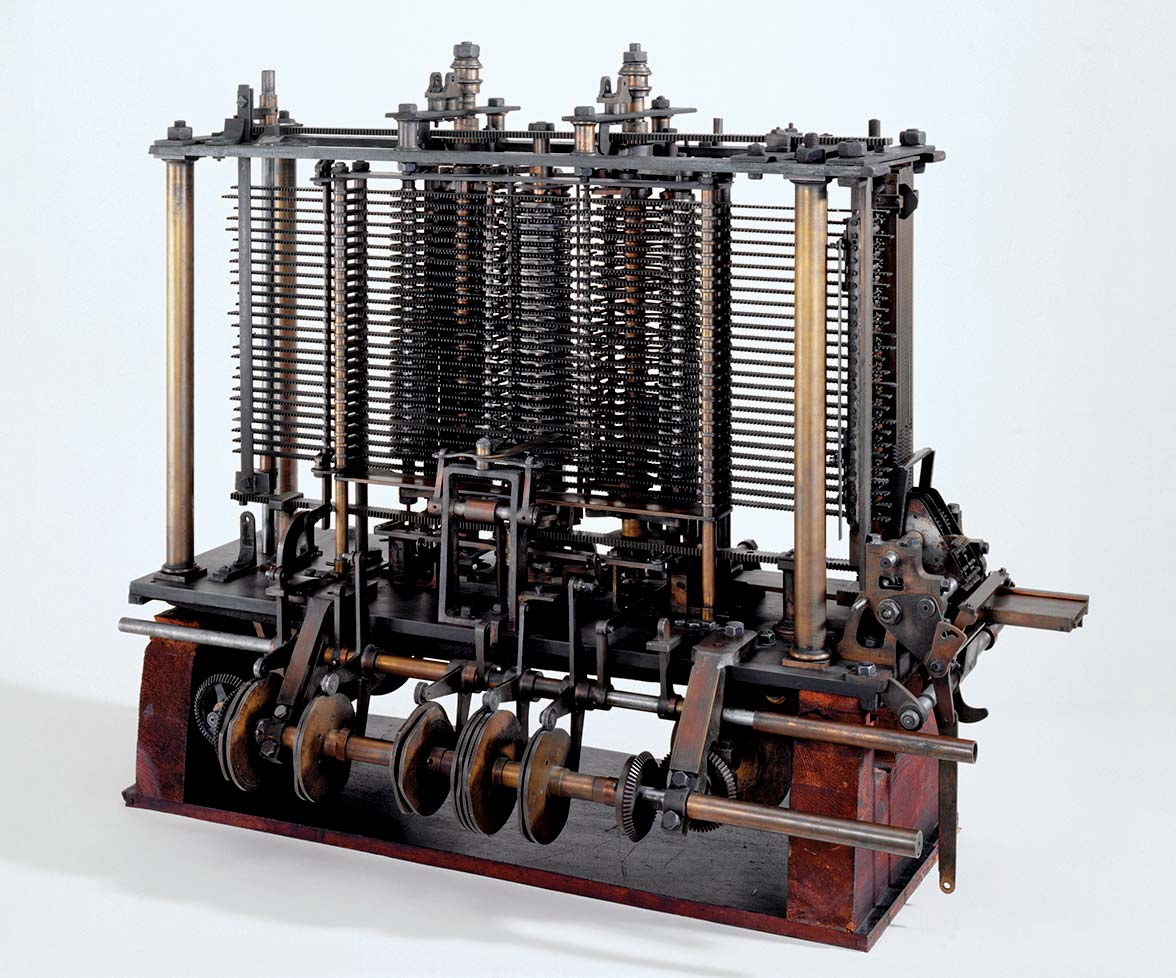
\includegraphics[width=0.2\textwidth]{portion-Charles-Babbage-Analytical-Engine-death-mill-1871.jpg}
\caption{The first general purpose computer, the Analytical Engine}
\label{fig:example}
\end{figure} 

In this form of the "computer", it is the relatively large components of mechanical gears and pegs which instantiate the logic of the underlying mathematics. Without a hint of modern electronic technology, logically meaningful instruction was stored in the macroscopic states of the wheels, which allow for the processing of input to output via mathematical rules. This incredible device was unfortunately left unfinished, but its design proved to be Turing-complete, essentially deeming the Analytic Engine as a true computer, an astonishing achievement for Victorian Age technology. 

\subsection{Vacuum Tube Technology}
With the prevalence of electricity-driven technology in the 20th century, it became possible to perform logical operations with the help of electronic components. Unlike the mechanically operated wheels of the Analytic Engine, electronic circuits allow for several orders-of-magnitude faster communications between hardware components. Vacuum Tubes along with their contemporaries, relay switches, are capable of storing memory states with the aid of electrical energy. Rather than storing the state of a logical operation in traditional physical form, vacuum tubes are advantageous for holding electrical energy, which can be received and transmitted almost instantly. 



\begin{figure}[h!]
\centering
\captionsetup{justification=centering}
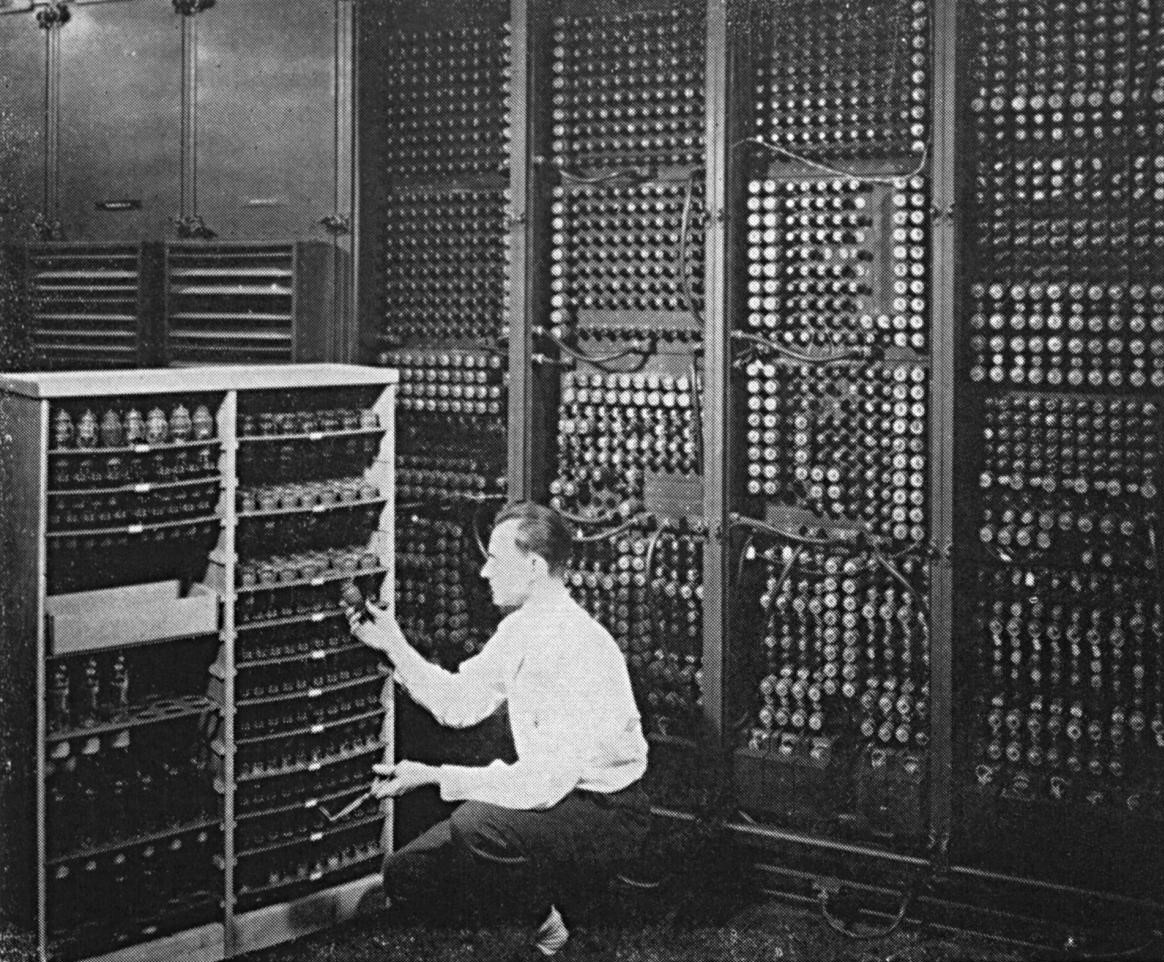
\includegraphics[width=0.2\textwidth]{ENIAC-changing_a_tube.jpg}
\caption{A technician changes a vacuum tube in the ENIAC}
\label{fig:example}
\end{figure} 



%Talk about the timeline from vacuum tube, 

\section{Integrated Circuit Revolution}

The creation of vacuum tubes has caused a revolutionary change in the history of computer hardware and made electronic computing possible for the first time but it also has major flaws that limit the capabilities of computing. Vacuum tubes are very hot, big, and uses a lot of electricity, the ENIAC also needed over 17,000 vacuum tubes for it to work in one discrete component. In 1947, transistors were becoming available and integrated into computers since they are better than vacuum tubes but they are built one at a time and wired together manually in a discrete component. To fix these flaws, Jack Kilby and Robert Noyce both independently created a new and reliable way of controlling electricity which is called integrated circuits in 1958. An integrated Circuit is an assembly of an electronic circuit formed with 5 transistors on a single IC in a few square millimeters at the start of the 1960s. Using photolithography and following Moore’s law, integrated circuits evolved into hundreds or thousands of transistors, and even resistors and capacitors were integrated. They can function as a vacuum tube but also an oscillator, timer, microprocessor, or even computer memory. This made an entire circuit integrated on one piece of material which made it better than vacuum tubes in size, voltage output, heat, and durability.

\subsection{Cost/Efficiency}

Although integrated circuits tackle most of the problems vacuum tubes faced, there are still limitations that integrated circuits can’t control. As integrated circuits are fixed, once a component is damaged, the whole integrated circuit must be replaced entirely unlike in a discrete circuit where a component can be replaced easily. It also can only handle a limited amount of power while power dissipation is limited to 10 watts 

\subsection{Moore's Law}

\begin{figure}[h!]
\centering
\captionsetup{justification=centering}
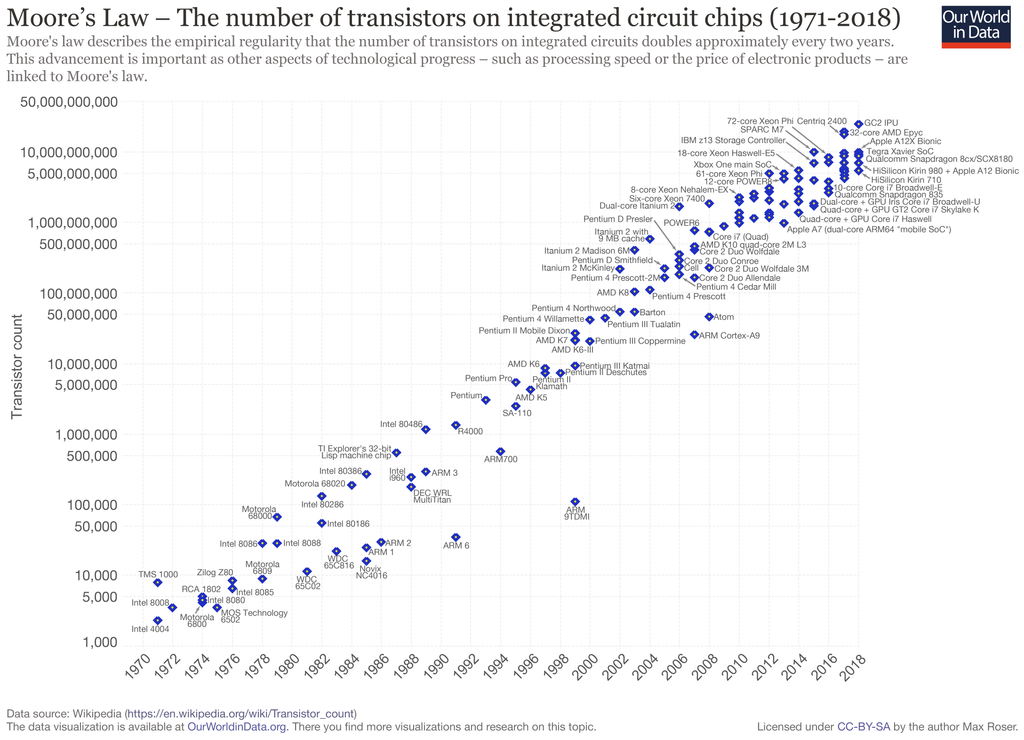
\includegraphics[width=0.2\textwidth]{1024px-Moore's_Law_Transistor_Count_1971-2018.png}
\caption{Integrated Circuit complexity over time, 1970-2018}
\label{fig:example}
\end{figure} 

Integrated circuits have gone through an immense growth per physical size over the years, leading to many of the breakthroughs enjoyed in modern technology.Starting in 1965, Gordon E. Moore, the co-founder of intel noticed a trend in the number of transistors in an integrated circuit every two years. Moore’s law states that as every two years pass, the number of transistors on a chip doubles, while the cost of these chips is halved. Although this trend is supposed to be a prediction, it became the driving force for the electronics industry to follow this trend

\section{CONCLUSION}

Conclude the ideas.

\section*{REFERENCES}


\begin{enumerate}[label={[\arabic*]}]
\item Rosen, Kenneth  H. Discrete Mathematics and Its Applications (Seventh Edition). McGraw-Hill, 2012. 
\item Woodford, Chris. “How Do Integrated Circuits Work?” Explain That Stuff, 30 Jan. 2020, www.explainthatstuff.com/integratedcircuits.html. 
\item Anysilicon. "The History of Integrated Circuit" anysilicon, 27 March 2020,
www.anysilicon.com/history-integrated-circuit/
\item "What is an Integrated Circuit (IC): Theory, Types of Integrated Circuits (Chips)" 27 February 2010. Retrieved from https://www.brighthubengineering.com/



\end{enumerate}

\end{document}


